
\section{Anforderungen}


Umschalten zwischen den beiden Spannungsquellen Netzteil und Akku nach folgendem Schema:
\begin{itemize}
	\item Wenn das Netzteil angeschlossen ist, dann soll dieses, unabhängig von der Akkuspannung, das System speisen. (FF)
	\item Wenn der Akkupack alleine angeschlossen ist, und dessen Spannung unter einen bestimmten Wert fällt, soll der Akku abgeschaltet werden, und keine Ausgangsspannung zur Verfügung gestellt werden. (WF)
	\item Zusätzlich soll eine Warnung ausgegeben werden, wenn die Akkuspannung unter eine bestimmte die Grenze fällt. Die Zeit bis zur Abschaltung muss ausreichen, "`stressfrei"' das Auto an das Netzteil zu hängen. Diese Warnung soll aber nur ausgegeben werden, wenn tatsächlich ein Akkupack eingesetzt ist. (FF)
	\item Dar Zustand soll in geeigneter Weise signalisiert werden. (WF)
\end{itemize}


\paragraph{Eigenschaften Verbraucher}
Der zulässige Bereich an Eingangsspannungen für das Mainboard ist \valunit{10}{V} bis \valunit{19}{V} (laut Händler) \bzw \valunit{8}{V} bis \valunit{19}{V} (laut Datenblatt).


\paragraph{Eigenschaften Netzteil}
Es handelt sich um ein Schaltnetzteil mit \valunit{12}{V} Nennspannung und \valunit{50}{W} Nennleistung.

Das verwendete Netzteil besitzt keine ausgeprägt höhere Leerlaufspannung. (Gemessen sind \valunit{12,15}{V} im Leerlauf, gegenüber \valunit{11,96}{V} bei ausgeschaltetem Rechner (Standby) und \valunit{12,14}{V} bei laufendem Rechner (ohne größere Prozessorlast,  mit baugleichem Netzteil).)


\paragraph{Eigenschaften Akkupack}
Es handelt sich um ein LiFe-Akkupack mit vier Zellen.

Das Akkupack kann Spannungen bis knapp unter \valunit{15}{V} ausweisen, wenn es gerade vom Ladegerät getrennt wird. (Die verwendete Schutzschaltung würde bei \valunit{15,6}{V} abschalten.)

Die Spannung im Betriebsbereich liegt zwischen \valunit{13,25}{V} und \valunit{12,5}{V} und ist von der Belastung abhängig. Der "`makroskopische"' Innenwiderstand (\dah nach Einschwingvorgängen) ist im Bereich von \valunit{65}{m\Omega} bis \valunit{100}{m\Omega} gemessen. Der "`instantane"' Innenwiderstand (direkte Spannungsänderung geteilt durch Stromänderung, ohne Einschwingvorgänge abzuwarten) beträgt \ca \valunit{30}{m\Omega.}

Bei \ca \valunit{9,2}{V} schaltet die Schutzschaltung ab, wobei es im Sinne einer längeren Lebensdauer auch sinnvoll wäre, den Akku vorher von der Last zu trennen. Die nominelle Entladeschlussspannung liegt (laut Wikipedia) bei \valunit{10}{V} bis \valunit{11,2}{V}.




\section{Abgeleitete Anforderungen}


\subsection{Spannungsgrenzen}

\paragraph{Netzteil}
\begin{itemize}
	\item Überspannung : \valunit{>14}{V}
	\item Unterspannung : \valunit{<9,5}{V} (> \vu{10,5}{V})
\end{itemize}

Die Überspannungsgrenze könnte prinzipiell auch auf \valunit{19}{V} gesetzt werden, da das Mainboard das aushält. Allerdings erhöht das den theoretisch möglichen Umschaltspitzenstrom erheblich, und eine Notwendigkeit, das System mit anderen Netzteilen als den ausgewählten verwenden zu können, besteht nicht.

Die Untergrenze ist auf \valunit{9,5}{V} gelegt, damit eine gewisse Reserve bezüglich einem Spannungseinbruch beim Umschalten auf das Netzteil besteht. Dies stellt auch die absolute Untergrenze dar, wenn man einen Spannungseinbruch von \vu{1}{V} während des Umschaltens am Ausgang zulässt. Durch die Unsicherheiten kann die tatsächliche Grenze auf \vu{9}{V} sinken, und damit besteht nur noch \vu{1}{V} Reserve zu der Mindestspannung von \vu{8}{V} des Rechners.

Die große Hysterese für die Untergrenze dient dazu, denn quellenseitigen Stützkondensator möglichst klein halten zu können.

%Es ist keine wesentliche Hysterese nötig, da Über- und Unterspannung außerhalb des normalen Betriebsbereiches des Netzteil liegen. Die Obergrenze schützt lediglich vor den verwenden eines falschen Netzteils, die Untergrenze wird nur beim "`Durchfallen"' der Ausgangsspannung erreicht, wenn am Netzstecker des Netzteils gezogen wird.


\paragraph{Akkupack}
\begin{itemize}
	\item Überspannung : \valunit{>15,5}{V} (\valunit{<15}{V})
	\item Unterspannung : \valunit{<10,5}{V} (\valunit{>11,5}{V})
\end{itemize}

Mit der Überspannungsgrenze von \valunit{15,5}{V} ist eine Verwendung von auch etwas sehr stark geladenen Akkus möglich. Die Untergrenze von \valunit{10,5}{V} liegt in der Mitte des nominellen Bereichs der Ladeschlussspannung und schützt den Akku vor zu tiefer Entladung. (Die \valunit{9,2}{V} des LiFe-Schützers sind schon sehr niedrig gewählt und schützen mehr vor Zerstörung als vor übermäßigen Verschleiß.) Testmessungen zeigen auch, dass man bei einer niedrigeren Grenze auch nicht viel Zeit gewinnt. (Bei \valunit{20}{W} ungefähr eine Minute, bei neuem Akku.)

Die Hysterese von \valunit{1}{V} soll sicherstellen, dass der Akku nicht wieder zugeschaltet wird, wenn sich die Akkuspannung im Leerlauf wieder erhöht. Testmessungen zeigen einen sehr deutlichen Anstieg der Ausgangsspannung des Akkus nach Abschalten der Last, wenn der Akku stark entladen ist. Dieser Anstieg ist umso größer, je größer der Entladestrom ist. Es ist auch mit der Hysterese von \valunit{1}{V} und höheren Entnahmeleistungen nicht ausgeschlossen, dass der Akku sich wieder zuschalten könnte. Letztlich betrifft das aber nur den Fall, dass der Akku abgeschaltet wurde und kein Netzteil angesteckt ist.

Größer kann die Hysterese nicht gewählt werden, da dann der Fall auftreten könnte, dass sich nach dem manuellen Ausschalten bei teilentladenen Akku es sich nicht mehr einschalten lässt. Dies wäre ein unerwünschtes Verhalten.



\paragraph{Warnung Akkupack}
\begin{itemize}
	\item Überspannung : $\infty$ (nicht überwacht)
	\item Unterspannung : \valunit{<12}{V} (\valunit{>12,25}{V})
\end{itemize}

Bei einer Warngrenze von \valunit{12}{V} und einer Abschaltgrenze von \valunit{10,5}{V} verbleiben bei \valunit{20}{W} Leistungsaufnahme ungefähr \valunit{5}{min} zwischen Warnung und Abschalten. Bei \valunit{60}{W} wären es noch \ca \valunit{2,5}{min}. (Jeweils am neuen Akku gemessen.) Dies reicht in allen Fällen für ein "`gemütliches"' Anstecken des Netzteils.


\subsection{Signalisierungen}

\begin{itemize}
	\item LED Netz: an, wenn "`Netz VALID"'
	\item LED Akku: an, wenn "`Akku VALID"'
	\item LED Akkuwarnung: an, wenn "`Akkutest $\mrm{\overline{VALID}}$"' und "`Akku VALID"'
	\item LED groß, blinkend und Summer Akkuwarnung: an, wenn "`Akkutest $\mrm{\overline{VALID}}$"' und "`Netz $\mrm{\overline{VALID}}$"'\\
		\begin{itemize}
			\item Es muss nicht zusätzlich überprüft werden, ob "`Akku VALID"' ist. Sollte dies nicht der Fall sein, stünde gar keine Spannung zur Verfügung, und damit würde auch keine Warnung signalisiert werden.
			\item Die Elemente Blink-LED und Summer müssen nur für den Spannungsbereich zwischen der Unterspannungsgrenze des Akkus und der Unterspannungsgrenze der Akkuwarnung spezifiziert sein. (Dies ist wesentlich, da viele in Frage kommenden Bauteile bis \valunit{14}{V} geeignet sind, und damit nicht an allen zulässigen Akku- und Netzteilspannungen betrieben werden dürfen.)
		\end{itemize}
\end{itemize}






\section{Auslegung}


\subsection{Spannungsgrenzen}


\subsubsection{Gleichungen}


Es werden die Bauteilbenennungen aus \figref{fig:OVUVSchematic} verwendet.

\begin{figure}[htb]%
	\centering
	\begin{tikzpicture}
		\ctikzset {label/align = straight}
		\draw[color=black, thick]
			(-2,0) to [short,o-] (0,0)
				to [short,-] (0,-1)
				to [R,-*,l_=$R_\mrm{t}$] (0,-3)
				to [R,-*,l_=$R_\mrm{m}$] (0,-5)
				to [R,-,l_=$R_\mrm{b}$] (0,-7) node[rground] {}
				%to node[rground]{} (0,-8)
			(0,-3) to [R,-*,l_=$R_\mrm{u}$] (2,-3)
				to [short,-o] (4,-3)
			(0,-5) to [R,-*,l_=$R_\mrm{o}$] (2,-5)
				to [short,-o] (4,-5)
			(2,-1) to [current source,-,i=$I_\mrm{u}$] (2,-3)
			(2,-7) to [current source,-,i_=$I_\mrm{o}$] (2,-5)
			(-2,-1) to [short,o-] (-1.5,-1)
				to [short,-] (-1.5,-1.25) node[rground,scale=0.5]{}
			(4,-4) to [short,o-] (3.5,-4)
				to [short,-] (3.5,-4.25) node[rground,scale=0.5]{}
			(4,-6) to [short,o-] (3.5,-6)
				to [short,-] (3.5,-6.25) node[rground,scale=0.5]{}
			;
		\draw[->, thick] (-2,-0.2) -- node [auto,swap] {$U_\mrm{in}$} (-2,-0.8);
		\draw[->, thick] (4,-3.2) -- node [auto] {$U_\mrm{comp,u}$} (4,-3.8);
		\draw[->, thick] (4,-5.2) -- node [auto] {$U_\mrm{comp,o}$} (4,-5.8);
	\end{tikzpicture}
	\caption{Schaltplan zur Festlegung der OV/UV-Grenzen}%
	\label{fig:OVUVSchematic}%
\end{figure}		


\begin{align*}
	I_\mrm{o} = I_\mrm{o,leak} \quad (\ + I_\mrm{hys} \ ) \\
	I_\mrm{u} = I_\mrm{u,leak} \quad (\ - I_\mrm{hys} \ )
\end{align*}

\begin{align*}
	I_\mrm{hys} = \frac{\valunit{63}{mV}}{R_\mrm{hys}}
\end{align*}


\begin{align*}
	U_\mrm{in,o} = \frac{R_\mrm{t} + R_\mrm{m} + R_\mrm{b}}{R_\mrm{b}} \cdot U_\mrm{comp,o} - R_\mrm{t} \cdot I_\mrm{u} - \left( R_\mrm{t} + R_\mrm{m} + \frac{R_\mrm{o} \cdot (R_\mrm{t} + R_\mrm{m} + R_\mrm{b})}{R_\mrm{b}} \right) \cdot I_\mrm{o}
\end{align*}


\begin{align*}
	U_\mrm{in,u} = \frac{R_\mrm{t} + R_\mrm{m} + R_\mrm{b}}{R_\mrm{m} + R_\mrm{b}} \cdot U_\mrm{comp,u} - \left( R_\mrm{t} + \frac{R_\mrm{u} \cdot (R_\mrm{t} + R_\mrm{m} + R_\mrm{b})}{R_\mrm{m} + R_\mrm{b}} \right) \cdot I_\mrm{u} - \frac{R_\mrm{t} R_\mrm{b}}{R_\mrm{m} + R_\mrm{b}} \cdot I_\mrm{o}
\end{align*}


Für die Nominalpunkte ergibt sich
\begin{align*}
	U_\mrm{ov} & = \frac{R_\mrm{t} + R_\mrm{m} + R_\mrm{b}}{R_\mrm{b}} \cdot \valunit{1}{V} \\
	U_\mrm{uv} & = \frac{R_\mrm{t} + R_\mrm{m} + R_\mrm{b}}{R_\mrm{m} + R_\mrm{b}} \cdot \valunit{1}{V}
\end{align*}

\begin{align*}
	U_\mrm{ov,hys} & = \left( R_\mrm{t} + R_\mrm{m} + \frac{R_\mrm{o} \cdot (R_\mrm{t} + R_\mrm{m} + R_\mrm{b})}{R_\mrm{b}} \right) \cdot I_\mrm{hys} \\
	U_\mrm{uv,hys} & = \left( R_\mrm{t} + \frac{R_\mrm{u} \cdot (R_\mrm{t} + R_\mrm{m} + R_\mrm{b})}{R_\mrm{m} + R_\mrm{b}} \right) \cdot I_\mrm{hys}
\end{align*}



\subsubsection{Festlegung der Bauteilwerte}

\paragraph{Hysteresestrom}

Da für den Akku eine sehr große Hysterese von \valunit{2}{V} vorgesehen ist, wird der höchstmögliche Hysteresestrom von \valunit{500}{nA} gewählt. Mit der Wahl
\begin{align*}
	R_\mrm{hys} = \vu{127}{k\Omega}
\end{align*}
ergibt sich 
\begin{align*}
	I_\mrm{hys} = \frac{\vu{63}{mV}}{\vu{127}{k\Omega}} = \vu{496,1}{nA}
\end{align*}



\paragraph{Grenzen Netzteil}

Wegen der großen Hysterese ist die "`Doppel-T-Struktur"' aus dem Datenblatt verwendet, die für diese Fälle empfohlen ist. Dabei besteht ein Freiheitsgrad, der hier mit der Wahl von $R_\mrm{t} = \valunit{200}{k\Omega}$ weggenommen ist. (Dieser Wert orientiert sich an den Werten in den Beispielschaltungen im Datenblatt.)


Mit
\begin{align*}
	R_\mrm{t} & = \vu{200}{k\Omega} &
	R_\mrm{m} & = \vu{8,45}{k\Omega} &
	R_\mrm{b} & = \vu{15,0}{k\Omega} &
	R_\mrm{u} & = \vu{200}{k\Omega} &
	R_\mrm{o} & = \vu{20,0}{k\Omega}
\end{align*}
erhält man
\begin{align*}
	U_\mrm{ov} & = \vu{14,90}{V} &
	U_\mrm{ov,hys} & = \vu{0,2512}{V} &
	\qquad ( \ U_\mrm{ov} - U_\mrm{ov,hys} & = \vu{14,65}{V} \ )
\end{align*}
sowie
\begin{align*}
	U_\mrm{uv} & = \vu{9,529}{V} &
	U_\mrm{uv,hys} & = \vu{1,045}{V} &
	\qquad ( \ U_\mrm{uv} + U_\mrm{uv,hys} & = \vu{10,57}{V} \ )\;.
\end{align*}




\paragraph{Grenzen Akku}

Wegen der großen Hysterese ist die "`Doppel-T-Struktur"' aus dem Datenblatt verwendet, die für diese Fälle empfohlen ist. Dabei besteht ein Freiheitsgrad, der hier mit der Wahl von $R_\mrm{t} = \valunit{200}{k\Omega}$ weggenommen ist. (Dieser Wert orientiert sich an den Werten in den Beispielschaltungen im Datenblatt.)

Mit
\begin{align*}
	R_\mrm{t} & = \vu{200}{k\Omega} &
	R_\mrm{m} & = \vu{6,80}{k\Omega} &
	R_\mrm{b} & = \vu{14,3}{k\Omega} &
	R_\mrm{u} & = \vu{174}{k\Omega} &
	R_\mrm{o} & = \vu{51,0}{k\Omega}
\end{align*}
erhält man
\begin{align*}
	U_\mrm{ov} & = \vu{15,46}{V} &
	U_\mrm{ov,hys} & = \vu{0,4938}{V} &
	\qquad ( \ U_\mrm{ov} - U_\mrm{ov,hys} & = \vu{14,97}{V} \ )
\end{align*}
sowie
\begin{align*}
	U_\mrm{uv} & = \vu{10,48}{V} &
	U_\mrm{uv,hys} & = \vu{1,004}{V} &
	\qquad ( \ U_\mrm{uv} + U_\mrm{uv,hys} & = \vu{11,48}{V} \ )\;.
\end{align*}



\paragraph{Grenzen Akkuwarnung}

Mit
\begin{align*}
	R_\mrm{t} & = \vu{200}{k\Omega} &
	R_\mrm{m} & = \vu{18,2}{k\Omega} &
	R_\mrm{b} & = \vu{0}{\Omega} &
	R_\mrm{u} & = \vu{0}{\Omega} &
	R_\mrm{o} & = \vu{0}{\Omega}
\end{align*}
erhält man
\begin{align*}
	U_\mrm{uv} & = \vu{11,99}{V} &
	U_\mrm{uv,hys} & = \vu{0,0992}{V} &
	\qquad ( \ U_\mrm{uv} + U_\mrm{uv,hys} & = \vu{12,09}{V} \ )\;.
\end{align*}



\subsubsection{Unsicherheitsanalyse}

Im Datenblatt sind mögliche Leckströme von
\begin{align*}
	I_\mrm{\{o,\,u\},leak} = \vu{\pm 20}{nA}
\end{align*}
angegeben. Dazu besitzen die Spannungskomperatoren eine Unsicherheit von \vu{pm 1,5}{\%},
\begin{align*}
	\Delta U_\mrm{comp,\{o,\,u\}} = \vu{\pm 1,5}{\%}\;.
\end{align*}

Geht man dazu noch von einer Unsicherheit von \vu{1}{\%} für $I_\mrm{hys}$ aus (um diese Unsicherheit gering zu halten, wird für $R_\mrm{hys}$ ein \vu{0,1}{\%}-Widerstand verwendet), kann die Unsicherheit der sich ergebenden Spannungsschwellen bestimmt werden.

In \figref{fig:OVUVLimits} ist für jede Schwelle der Bereich der Unsicherheit eingetragen. Zusätzlich zu den oben angegebenen Unsicherheiten sind dabei noch die Unsicherheiten der Widerstände berücksichtigt. Dabei sind \vu{1}{\%}-Widerstände (dünne Balken) sowie \vu{0,1}{\%}-Widerstände (dünne Balken) berücksichtigt.

\begin{figure}[htb]%
	\centering
	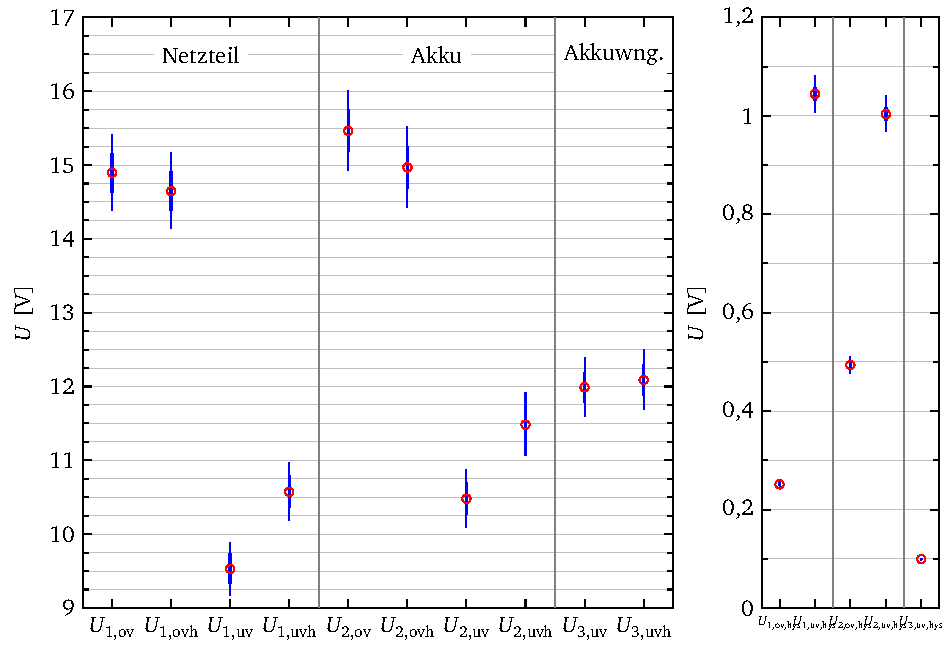
\includegraphics{tikz/ext/OVUVLimits-ext}%
	\caption{OV/UV-Grenzen mit Unsicherheit}%
	\label{fig:OVUVLimits}%
\end{figure}

Die Schwellen streuen \zT deutlich. Die Hysteresewerte sind jedoch relativ stabil.



\subsection{Leistungspfade}

Die "`Leistungspfade"' bestehen aus den Mosfets mit der optionalen Slew-Rate-Schaltung sowie den Ein- und Ausgangskondensatoren.

Abgesehen vom Einschalten (\dah vom Ausgangszustand, dass keine gültige Spannung anliegt) werden die Mosfets "`hart"' geschaltet. Dies kann zu realtiv großen Ausgleichsströmen führen. Neben der Überlastung der Mosfets können diese hohen Ströme auch Spannungseinbrüche der Spannungsquellen hervorrufen, die dazu führen, dass diese den gültigen Bereich verlassen und damit wieder abgeschaltet werden.



Prinzipiell gibt es zwei Möglichkeiten:
\begin{itemize}
	\item "`Überdimensionierte"' Mosfets, die auch große Pulsströme überleben. Dann kann auf die Slew-Rate-Schaltung verzichtet werden.
	\item Mosfets, die sich am Dauerstrom orientieren.
\end{itemize}



\paragraph{Ausgangskondensator}

Der Ausgangskondensator muss für die Zeit der Umschaltung den Rechner speisen. Die Ausgangsspannung während der Umschaltung soll um maximal \vu{1}{V} absinken. Geht man von einem ESR von \vu{50}{m\Omega} des Ausgangskondensators aus, ergibt sich bei \vu{5}{A} ein Spannungsabfall von \vu{250}{mV} im Kondensator. Damit beträgt der maximal zulässige Spannungsabfall aufgrund der Entladung \vu{750}{mA}. Die Kapazität des Ausgangskondensators muss damit die Bedingung
\begin{align*}
	C_\mrm{L} \geq \frac{\valunit{5}{A} \cdot (\valunit{3}{\upmu s} + \valunit{13}{\upmu s} + \Delta t_\mrm{slewrate})}{\valunit{750}{mV}}
\end{align*}
erfüllen, wobei die $\valunit{3}{\upmu s} + \valunit{13}{\upmu s}$ "`systemimmanente"' Umschaltzeit, die überbrückt werden muss, ist. $\Delta t_\mrm{slewrate}$ ist die zusätzliche Zeit aufgrund der optionalen Slew-Rate-Schaltung und wird nach Datenblatt über
\begin{align*}
	\Delta t_\mrm{slewrate} = 0,79 \cdot R_\mrm{S} C_\mrm{S}
\end{align*}
berechnet.



\paragraph{Eingangskondensator}


Im Datenblatt ist für den Eingangskondensator die Bedingung
\begin{align*}
	C_\mrm{U1} \geq C_\mrm{L} \cdot \left(\frac{U_1 - U_\mrm{out(init)}}{U_\mrm{1,droop}} - 1 \right)
\end{align*}
angegeben. Diese ergibt sich aus der Eingangsspannung $U_1$ zum Zeitpunkt des Einschaltens der Spannungsquelle 1, der Ausgangsspannung $U_\mrm{out(init)}$ zum Zeitpunkt des Einschaltens und dem zulässigen Spannungseinbruch $U_\mrm{1,droop}$ der Spannungsquelle 1. (Die Gleichung basiert auf der Betrachtung des Umladevorgangs von zwei parallelgeschalteten Kondensatoren.)


\paragraph{Eingangskondensator -- Netzteil}

Als einziges Kriterium wird hier erachtet, dass die Spannungsquelle 1 sich nicht direkt wieder abschalten darf, weil die Unterspannungsbedingung vorliegt. \Dah
\begin{align*}
	U_\mrm{1,droop} = U_1 - U_\mrm{1,uv}\;.
\end{align*}
Damit erhält man
\begin{align*}
	\frac{C_\mrm{U1}}{C_\mrm{L}} \geq \frac{U_1 - U_\mrm{out(init)}}{U_1 - U_\mrm{1,uv}} - 1\;.
\end{align*}

Der kritische Fall ist hier, wenn das Netzteil durch Einstecken des Netzsteckers eingeschaltet wird. Die Spannung läuft dann "`langsam"' hoch, und $U_1 - U_\mrm{1,uv}$ entspricht gerade der Hysterese $U_\mrm{1,uv,hys}$.

Die niedrigste Spannung $U_\mrm{out(init)}$ tritt auf, wenn der Akku kurz vor der Unterspannungsschwelle steht. Von dieser müssen dann noch die \vu{0,75}{V} abgezogen werden, die die Spannung von $C_\mrm{L}$ während des Umschaltvorgangs fallen darf.

Somit ergibt sich
\begin{align*}
	U_1 & = U_\mrm{1,uv} + U_\mrm{1,uv,hys} = \vu{10,75}{V} \\
	U_1 - U_\mrm{1,uv} & = U_\mrm{1,uv,hys} = \vu{1}{V} \\
	U_\mrm{out(init)} & = \vu{10}{V} - \vu{0,75}{V} = \vu{9,25}{V}.
\end{align*}

\begin{align*}
	\frac{C_\mrm{U1}}{C_\mrm{L}} \geq 0,5
\end{align*}



\paragraph{Eingangskondensator -- Akku}


\begin{align*}
	\frac{C_\mrm{U2}}{C_\mrm{L}} \geq \frac{U_2 - U_\mrm{out(init)}}{U_2 - U_\mrm{2,uv}} - 1\;.
\end{align*}




\begin{align*}
	U_2 & = U_\mrm{2,uv} + U_\mrm{2,uv,hys} = \vu{12}{V} \\
	U_2 - U_\mrm{2,uv} & = U_\mrm{2,uv,hys} = \vu{1}{V} \\
	U_\mrm{out(init)} & = \vu{9}{V} - \vu{0,75}{V} = \vu{8,25}{V}.
\end{align*}


\begin{align*}
	\frac{C_\mrm{U2}}{C_\mrm{L}} \geq 2,75
\end{align*}


Bei einer Strombegrenzung auf \vu{35}{A} und einem Innenwiderstand des Akkus von \vu{30}{m\Omega} ergibt sich ein Spannungsabfall von \vu{1,05}{V}. Damit kann sich der Akku in der Regel selber über der Unterspannungsgrenze halten und ein Kondensator ist nicht nötig.



\subsubsection{Mosfet}


\paragraph{"`Schwacher"' Mosfet}
\begin{itemize}
	\item Typ: TPC8120
	\item $V_\mrm{GS,min} = \valunit{-25}{V}$, $V_\mrm{GS,max} = \valunit{20}{V}$
	\item $I_\mrm{D,maxPulse} = \valunit{-72}{A}$
	\item $I_\mrm{D,max} = \valunit{-18}{A}$
	\item $R_\mrm{DS(on)} = \valunit{3,3}{m\Omega}$ bei $V_\mrm{GS} = \valunit{-4,5}{V}$ \\
				$R_\mrm{DS(on)} = \valunit{2,6}{m\Omega}$ bei $V_\mrm{GS} = \valunit{-10}{V}$
	\item $V_\mrm{GS(th),max} = \valunit{-0,8}{V}$, $V_\mrm{GS(th),min} = \valunit{-2}{V}$
	\item $C_\mrm{RSS,max} = \valunit{1,18}{nF}$
\end{itemize}



\subsection{Einschaltstrombegrenzung und Pufferkondensator}

Da die Eingangsbeschaltung des Boards nicht bekannt ist, kann hierfür kein Widerstand angegeben werden. Der Worst-Case ist ein geringer Widerstand, so dass dieser auf null gesetzt wird.

\begin{align*}
	R_\mrm{inrush} = R_\mrm{source} + R_\mrm{fets} + (R_\mrm{CL} || R_\mrm{pc,in})
\end{align*}

\begin{align*}
	R_\mrm{fets} = 2 \cdot R_\mrm{DS(on)} = \valunit{5,2}{m\Omega}
\end{align*}

$R_\mrm{CL}$ ist der ESR des Ausgangskondensators der Schaltung und sollte über einen geringen ESR verfügen. 



\paragraph{Umschalten von Akku auf Netzteil}

Der worst-case Spannungssprung ist von der niedrigsten Akkuspannung minus dem Spannungsabfall während des Umschaltens ($\vu{10}{V} - \vu{1}{V} = \vu{9}{V}$) auf die höchste Netzteilspannung (\valunit{15,25}{V}), also \valunit{6,25}{V}.

\begin{align*}
	R_\mrm{source} = \valunit{10}{m\Omega}
\end{align*}

\begin{align*}
	R_\mrm{inrush} = \valunit{20,2}{m\Omega}
\end{align*}

\begin{align*}
	I_\mrm{inrush} = \frac{\valunit{6,25}{V}}{\valunit{20,2}{m \Omega}} = \valunit{309}{A}
\end{align*}


\paragraph{Umschalten von Netzteil auf Akku}

Der worst-case Spannungssprung ist von der niedrigsten Netzteilspannung minus dem Spannungsabfall während des Umschaltens ($\vu{9}{V} - \vu{1}{V} = \vu{8}{V}$) auf die höchste Akkuspannung (\valunit{16}{V}), also \valunit{8}{V}.

\begin{align*}
	R_\mrm{source} = \valunit{30}{m\Omega}
\end{align*}

\begin{align*}
	R_\mrm{inrush} = \valunit{40,2}{m\Omega}
\end{align*}

\begin{align*}
	I_\mrm{inrush} = \frac{\valunit{8}{V}}{\valunit{40,2}{m \Omega}} = \valunit{199}{A}
\end{align*}




\subsubsection{Rechnungen "`kleiner Mosfet"'}

Der Kondensator $C_\mrm{S}$ der Slew-Rate-Schaltung wir laut Datenblatt zu
\begin{align*}
	C_\mrm{S} = 10 \cdot C_\mrm{RSS} \approx \valunit{12}{nF} 
\end{align*}
gewählt.

Mit einem maximalen Pulsstrom von
\begin{align*}
	I_\mrm{inrush} = \valunit{35}{A}
\end{align*}
ergibt sich nach dem iterativen Vorgehen aus dem Datenblatt letztlich
\begin{align*}
	C_\mrm{L} = \valunit{470}{\upmu F}
\end{align*}
und
\begin{align*}
	R_\mrm{S} \geq 
		\frac{(\Delta V_\mrm{G(sink)} - V_\mrm{GS}) \cdot 1,2 \cdot C_\mrm{L}}{C_\mrm{S} \cdot I_\mrm{tot}}
		= \frac{(\valunit{6}{V} - \valunit{2}{V}) \cdot \valunit{564}{\upmu F}}{\valunit{12}{nF} \cdot \valunit{35}{A}}
		= \valunit{5,4}{k\Omega}\;.
\end{align*}
Mit der Wahl
\begin{align*}
	R_\mrm{S} = \valunit{5,6}{k\Omega}
\end{align*}
ergibt sich mit
\begin{align*}
	 0,79 \cdot R_\mrm{S} C_\mrm{S} = 0,79 \cdot \valunit{5,6}{k\Omega} \cdot \valunit{12}{nF} = \valunit{53}{\upmu s}
\end{align*}
die Bedingung
\begin{align*}
	C_\mrm{L} \geq \frac{\valunit{5}{A} \cdot (\valunit{3}{\upmu s} + \valunit{13}{\upmu s} + \valunit{53}{\upmu s})}{\valunit{750}{mV}} = \valunit{460}{\upmu F}
\end{align*}
für das minimale $C_\mrm{L}$, welche mit $C_\mrm{L} = \valunit{470}{\upmu F}$ erfüllt ist.




\paragraph{Eingangskondensator}





\subsubsection{Rechnungen "`großer Mosfet"'}

Der Ausgangskondensator muss die Bedingung
\begin{align*}
	C_\mrm{L} \geq \frac{\valunit{5}{A} \cdot (\valunit{3}{\upmu s} + \valunit{13}{\upmu s})}{\valunit{750}{mV}} = \valunit{107}{\upmu F}
\end{align*}
erfüllen. Der nächste Standardtyp (mit etwas Auswahl bei der Spannungsfestigkeit) ist
\begin{align*}
	C_\mrm{L} = \vu{150}{\upmu F}\;.
\end{align*}




